\chapter{Results}\label{CH_04}

\section{Binning in redshift}
Stellar mass density is calculated within some volume, so we bin our sample to four redshift intervals of the same comoving volume - $139,729,000 Mpc^{3}$. The size of the bin is chosen the way that we still have sufficient sources in the highest redshift bin that goes up to z=0.8 - even though our photometric redshifts span up to $z\approx~0.9$, the number sources at this redshift decreases significantly and this incompleteness leads to the severe underestimation of the number density. Information about binning is presented in Table~\ref{tab:redshift_bin}. Although it is tempting to create larger number of bin in order to see evolution of the stellar mass at "high-resolution", we remember that our redshift is determined based on photometry and thus is not reliable within better than $\Delta z\approx 0.1-0.15$ (also recall large scatter around $z\sim0.4$). So we decide to have four large bins in which errors in redshifts and associated stellar masses shall be averaged. Stellar mass is plotted against z\_phot in all four bins on Figure~\ref{fig:sm_z_dissect}.

\begin{figure}[!ht]
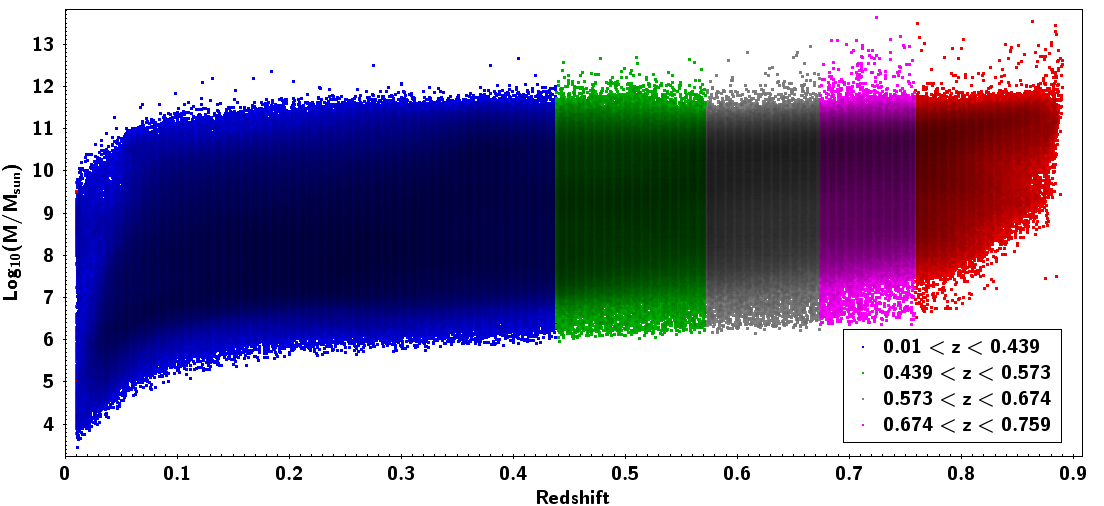
\includegraphics[width=6in]{Figures/mass_vs_photo_z_dissected.png}
\caption{Stellar mass density over photometric redshift. Four reddshift bins are plotted in different colors: z1 - blue, z2 - green, z3 - grey, z4 - magenta. Red sources at z$>$0.759 are not included into the sample due to their low number density.}
\label{fig:sm_z_dissect}
\end{figure}

\begin{table}[h!]
  \begin{center}
    \caption{Redshift binning of stellar mass}
    \begin{tabular}{l|l|l|l|l} % <-- Changed to S here.
     \textbf{\#} & \textbf{redshift} & \textbf{mean} & \textbf{\# of galaxies} & \textbf{fraction of galaxies}\\
     \textbf{} & \textbf{interval} & \textbf{redshift} & \textbf{per bin} & \textbf{per bin}\\
%      $\alpha$ & $\beta$ & $\gamma$ \\
      \hline
%      aperture [pix] & ?? & ?? & ?? & ?? & ??\\
      1 & 0.010$<z>$0.439 & 0.296 & 6,065,140 & 0.65\\
      2 & 0.439$<z<$0.573 & 0.506 & 1,588,509 & 0.17\\
      3 & 0.573$<z<$0.674 & 0.623 & 812,562  & 0.09\\
      4 & 0.674$<z<$0.759 & 0.716 & 585,009  & 0.06\\
    \end{tabular}
  \end{center}
  \label{tab:redshift_bin}
\end{table}

We sum up stellar mass of all galaxies in a bin and divide it by the bin volume to derive the stellar mass density per bin in units of $M_{\odot}/Mpc^{3}$. Stellar mass density is usually represented in a log scale. Also, in order to compare our results to other published data we scaled from a Chabrier IMF to a Salpeter IMF by multiplying the stellar masses by a factor of 1.64. Results are combined in Table~\ref{tab:smd} and will be published in \cite{Musin2018}.

\begin{table}[h!]
  \begin{center}
    \caption{Stellar mass density}
    \begin{tabular}{l|l|l|l|l|l|l} % <-- Changed to S here.
     \textbf{redshift} & \textbf{light-travel} & \textbf{total mass} & \text{total mass} & \textbf{$Log_{10}(\rho)$} & \textbf{$Log_{10}(\rho)$}\\
     \textbf{interval} & \textbf{time interval}          & \textbf{BC03} & \text{MA11} & \textbf{Chabrier IMF} & \textbf{Salpeter IMF}\\
	  \hline
       z & Gyr & $M_{\odot}$ & $Log_{10}(M_{\odot}/Mpc^{3})$ & $Log_{10}(M_{\odot}/Mpc^{3}$)\\
      \hline
      0.010$<z<$0.439 & 0.139-4.589 & $2.76\cdot 10^{16}$ & $2.72\cdot 10^{16}$ & 8.299 & 8.514\\
      0.439$<z<$0.573 & 4.589-5.537 & $1.89\cdot 10^{16}$ & $1.85\cdot 10^{16}$ & 8.077 & 8.292\\
      0.573$<z<$0.674 & 5.537-6.154 & $1.74\cdot 10^{16}$ & $1.52\cdot 10^{16}$ & 8.050 & 8.265\\
      0.674$<z<$0.759 & 6.154-6.619 & $1.74\cdot 10^{16}$ & $1.20\cdot 10^{16}$ & 8.089 & 8.304\\
    \end{tabular}
  \end{center}
  \label{tab:smd}
\end{table}

\begin{figure}[!ht]
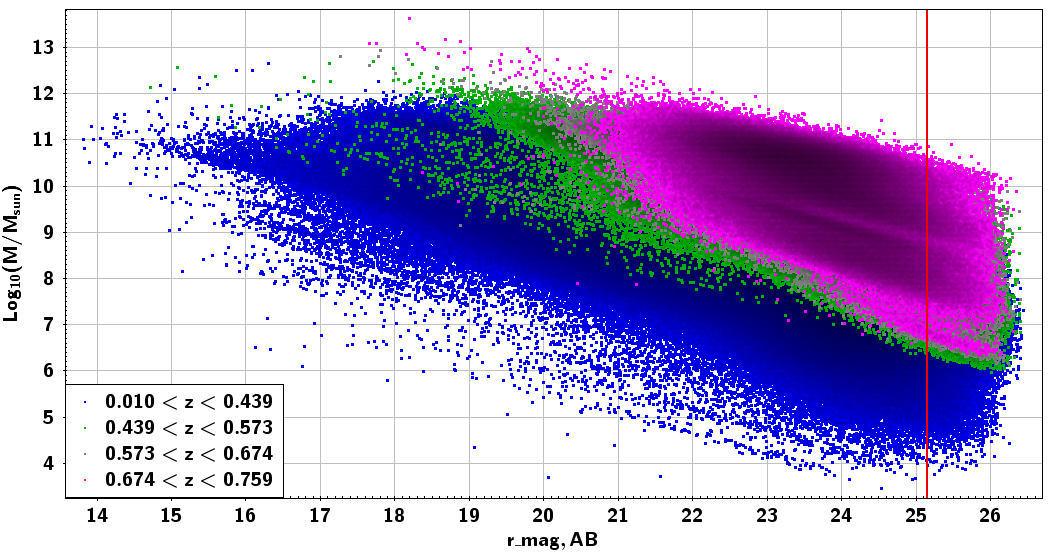
\includegraphics[width=6in]{Figures/mass_vs_r-mag.png}
\caption{Stellar masses are plotted over corresponding r-band magnitudes. Four redshift bins are plotted in different colors: z1 - blue, z2 - green, z3 - grey, z4 - magenta. Red vertical line denotes r-band $3\sigma$ detection limit.}
\label{fig:sm_mag_r}
\end{figure}

On the Figure~\ref{fig:sm_mag_r} we present stellar masses, binned to four redshifts as a function of r-band magnitude. Red vertical line shows the $3\sigma$ detection limit for the r-band. It does not necessarily mean that we should not trust masses beyond this limit as those sources may have reliable photometry in other bands, but it should at least be taken with caution.

\section{GSMD and comparison to the results of other groups}

In their review paper Madau \& Dickinson \citep{Madau2014} presented a compilation of recent measurements of SMD from different groups up to $z\approx 8$. They used all available data including wide field local SDSS based SMD. We predict that before any corrections our SMD should be somewhat close to reported results. We overplotted our derived SMD with red stars on top of the data presented in \citep{Madau2014}. As you may see on Figure~\ref{fig:gsmd_my} our points lie very close to some of the reported data, especially to \citep{2012A&A...545A..23B}, who used J,H and Ks filters to investigate the SMD in four CFHTLS deep fields.

Our reported mass density for the fourth redshift bin, 0.674$<z<$0.759 (8.089) is higher than that for the third one, 0.573$<z<$0.674 (8.050). It may not be a representation of any real processes, because even though generally stellar mass in a certain small volume can go down due to the end of the life cycle of massive stars, in general galaxies tend to increase their stellar mass in time. Interestingly, the same behavior is observed in the data of other groups, as can clearly be seen on Figure~\ref{fig:gsmd_my} in the region denoted by red rectangular. We interpret this "wiggle" in two ways - as a direct evidence of the incompleteness of our data sample or as a systematic overestimation of stellar masses in the highest redshift bin (some galaxies are assigned with stellar masses as high as $10^{13}M_{sun}$, which is not supported by any observations of galaxies at such redshifts. 

\begin{figure}[!ht]
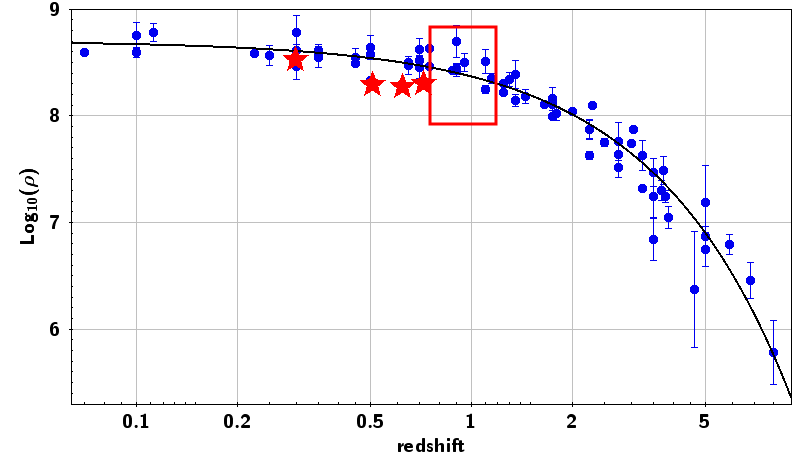
\includegraphics[width=6in]{Figures/md_plot_my_data_1.png}
\caption{Overplotted Figure 11 from Madau\&Dickinson 2014 with our SMD data points plotted as low-limit with with red stars. Data points inside the red rectangular demonstrate an odd "wiggle" upwards as if the SMD was higher in the earlier Universe. Black solid line is an approximation of the global stellar mass density obtained by integrating the best-fit instantaneous star-formation rate density}
\label{fig:gsmd_my}
\end{figure}

The problem of incompleteness appears in any survey, photometric or spectroscopic - low-mass galaxies at higher redshifts are too dim to be detected. Correction for incompleteness is beyond the scope of this thesis and we only outline here the possible approach. This incompleteness can be estimated based on a comparison to the much deeper small area surveys or based on the analytic correction that can be applied using the available data from Figure~\ref{fig:sm_z_dissect}.

